\documentclass{beamer}

% presentation themeing
\usetheme{Singapore}
\beamertemplatenavigationsymbolsempty
\setbeamertemplate{bibliography item}{\insertbiblabel}
\setbeamercovered{again covered={\opaqueness<1->{15}}}

% output configuration
\usepackage{pgfpages}
%\setbeameroption{show notes on second screen=left}
\hypersetup{pdfpagemode=FullScreen}

% type setting packages
\usepackage{algorithmic}
\usepackage{amsmath}
\usepackage{siunitx}
\usepackage{etoolbox}

%math typeseting
\newcommand{\mat}[1]{\mathbf{#1}}

% plotting setup
\usepackage{pgfplots}
	\pgfplotsset{compat=1.16}
\usepackage{pgfplotstable}
\usepgfplotslibrary{external} 
\tikzexternalize

\pgfplotstableset{col sep=semicolon}

\pgfplotstableread{figures/4.Results/Vec.csv}\vectable
\pgfplotstableread{figures/4.Results/Ind.csv}\indtable
\pgfplotstableread{figures/4.Results/Val.csv}\valtable

% title slide
\title{\input{title.txt}}
\subtitle{All-College Thesis Defense}
\author{\textbf{Neil Lindquist}}
\date{April 16th, 2019}

\begin{document}
\begin{frame}
	\titlepage
\end{frame}

% Motivation
\begin{frame}
	\frametitle{Motivation}
	\begin{itemize}
		\item Solving sparse linear systems used in many computations
		\item Iterative solvers are used
		\item Spend most of the time fetching data
	\end{itemize}
\end{frame}

\begin{frame}
	\frametitle{Mathematics of Conjugate Gradient}
	\begin{itemize}
		% mention that CG converges faster than other methods (SOR et al)
		\item Solving \(\mat{A}\vec{x} = \vec{b}\)
		\pause
		\item Minimizing \(f(\vec{x}) = \tfrac{1}{2}\vec{x}^T\mat{A}\vec{x}-\vec{b}\cdot\vec{x}\)
		\pause
		\item If \(\mat{A}\) is symmetric, then \(\nabla f(\vec{x}) = \mat{A}\vec{x} - \vec{b}\)
		\pause
		\item \(-\nabla f(\vec{x})\) is in direction of maximal decrease
	\end{itemize}
\end{frame}

\begin{frame}
	\frametitle{Mathematics of Conjugate Gradient}
	\centering
	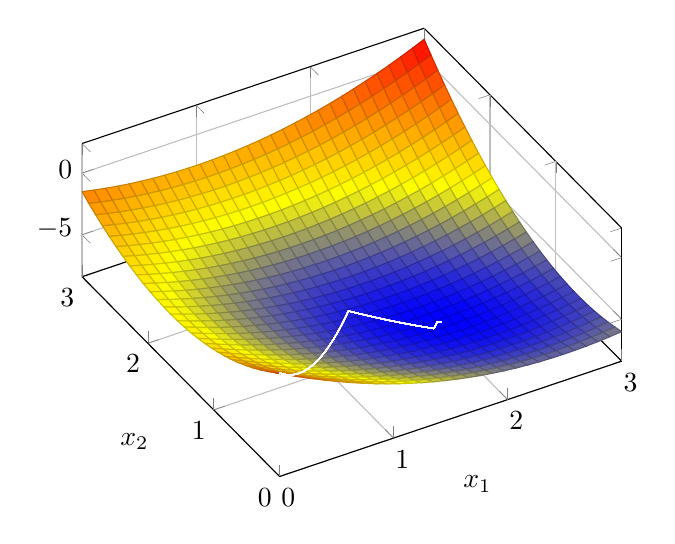
\begin{tikzpicture}
		\begin{axis}[
				grid=major,
				view={-30}{60},
				xlabel=\(x_1\),
				ylabel=\(x_2\),
				samples=30,
				]
			\addplot3[surf,domain=0:3] 
				{.5*(2*x^2 + 2*x*y + 3*y^2) - 5*x - 5*y};
			\addplot3[mesh,domain=0:10/7,color=white] 
				({x},{x}, {.5*(2*x^2 + 2*x*x + 3*x^2) - 5*x - 5*x});
			\addplot3[mesh,domain=0:1,color=white] 
				({(10/21)*x+10/7},{(-10/21)*x+10/7},
				{.5*(2*((10/21)*x+10/7)^2 + 2*((10/21)*x+10/7)*((-10/21)*x+10/7) + 3*((-10/21)*x+10/7)^2) - 5*((10/21)*x+10/7) - 5*((-10/21)*x+10/7)});
			\addplot3[mesh,domain=0:1,color=white] 
				({(10/147)*x+40/21},{(10/147)*x+20/21},
				{.5*(2*((10/147)*x+40/21)^2 + 2*((10/147)*x+40/21)*((10/147)*x+20/21) + 3*((10/147)*x+20/21)^2) - 5*((10/147)*x+40/21) - 5*((10/147)*x+20/21)});
			\addplot3[mesh,domain=0:1,color=white] 
				({(10/441)*x+290/147},{(-10/441)*x+50/49},
				{.5*(2*((10/441)*x+290/147)^2 + 2*((10/441)*x+290/147)*((-10/441)*x+50/49) + 3*((-10/441)*x+50/49)^2) - 5*((10/441)*x+290/147) - 5*((-10/441)*x+50/49)});
%			\addplot3[mesh,domain=0:1,color=white] 
%				({(10/3087)*x + 880/441},{(10/3087)*x + 440/441},
%				{.5*(2*((10/3087)*x+880/441)^2 + 2*((10/3087)*x+880/441)*((10/3087)*x+440/441) + 3*((10/3087)*x+440/441)^2) - 5*((10/3087)*x+880/441) - 5*((10/3087)*x+440/441)});
		\end{axis}
	\end{tikzpicture}
\end{frame}

\begin{frame}
	\frametitle{Mathematics of Conjugate Gradient}
	\centering
	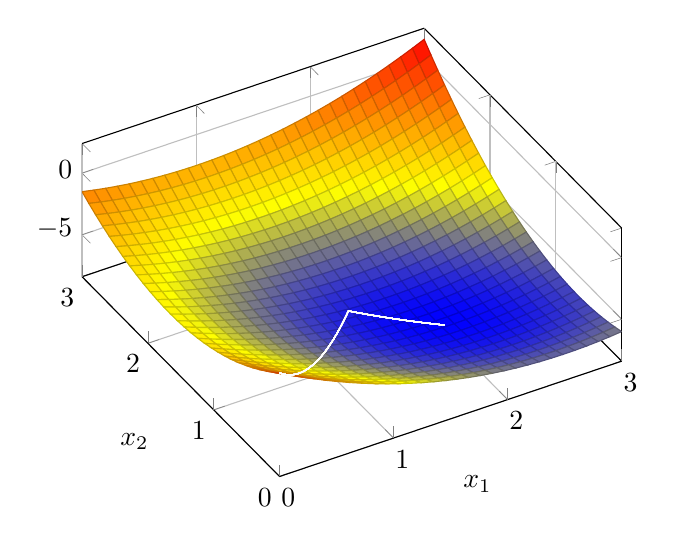
\begin{tikzpicture}
		\begin{axis}[
				grid=major,
				view={-30}{60},
				xlabel=\(x_1\),
				ylabel=\(x_2\),
				samples=30,
				]
			\addplot3[surf,domain=0:3] 
				{.5*(2*x^2 + 2*x*y + 3*y^2) - 5*x - 5*y};
			\addplot3[mesh,domain=0:10/7,color=white] 
				({x},{x}, {.5*(2*x^2 + 2*x*x + 3*x^2) - 5*x - 5*x});
			\addplot3[mesh,domain=0:1,color=white] 
				({(4/7)*x+10/7},{(-10/21)*x+10/7},
				{.5*(2*((4/7)*x+10/7)^2 + 2*((4/7)*x+10/7)*((-3/7)*x+10/7) + 3*((-3/7)*x+10/7)^2) - 5*((4/7)*x+10/7) - 5*((-3/7)*x+10/7)});
%			\addplot3[mesh,domain=0:1,color=white] 
%				({(10/3087)*x + 880/441},{(10/3087)*x + 440/441},
%				{.5*(2*((10/3087)*x+880/441)^2 + 2*((10/3087)*x+880/441)*((10/3087)*x+440/441) + 3*((10/3087)*x+440/441)^2) - 5*((10/3087)*x+880/441) - 5*((10/3087)*x+440/441)});
		\end{axis}
	\end{tikzpicture}
\end{frame}

% Data access patterns/compression limitations
\begin{frame}
	\frametitle{Solver Description}
	\begin{itemize}
		%TODO should this information be here?
		%just describe the matrix instead
		\item Approximating the steady state heat equation in 3 dimensions
		\begin{itemize}
			%\item \(0 = \frac{\partial}{\partial x}u(x, y, z) +\frac{\partial}{\partial y}u(x, y, z) + \frac{\partial}{\partial z}u(x, y, z)\)
			\item Discretized with a 27-point stencil
		\end{itemize}
		\pause
		\item Preconditioned Conjugate Gradient was used
		\begin{itemize}
			\item 3-level multigrid preconditioner with Symmetric Gauss-Seidel smoother
		\end{itemize}
		\pause
		\item Matrix store in CSR format
		\begin{itemize}
			\item Stores the column index and value for each nonzero entry
		\end{itemize}
		\pause
		\item 3 compressible data structures
		\begin{itemize}
			\item Vector Values
			\item Matrix Indices
			\item Matrix Values
		\end{itemize}
	\end{itemize}
\end{frame}

% Select Compression methods
\begin{frame}
	\frametitle{Compression Methods}
	\begin{itemize}
		\item<1-2> Mixed Floating Point Precision
		\item<1-2> SZ Compression
		\item<1-2> Elias Gamma and Delta Codings
		\item<1> ZFP Compression
		\item<1> Huffman Coding
		\item<1> Op Code Compression
	\end{itemize}
\end{frame}

\begin{frame}
	\frametitle{Mixed Floating Point Precision}
	\begin{itemize}
		\item Trade off between storage and precision
		\item Certain vectors can be lower precision without slowing convergence
		\begin{itemize}
			\item Retains result accuracy
		\end{itemize}
	\end{itemize}
\end{frame}

\begin{frame}
	\frametitle{Squeeze ``SZ'' Compression}
	\begin{itemize}
		\item Predicts each value from the previous few
		\item Enforces minimum accuracy
		\pause
		\item Available prediction functions are based on the data
		\pause
		\item Compression rate is highly dependent on local patterns in the data
	\end{itemize}
\end{frame}
%TODO consider adding an example

\begin{frame}
	\frametitle{Elias Gamma Coding}
	\begin{itemize}
		\item Positive integers
		\item For each value, stores the size then the data
		\begin{itemize}
			\item Very effective for small integers
			\item Storing the difference from the previous index reduces the size of values
		\end{itemize}
		\pause
		\item Elias Delta Coding is similar, but uses Gamma coding for the length
		\pause
		\item Compression rate is only dependent on the magnitude of the values
	\end{itemize}
\end{frame}

% Timing results
\begin{frame}
	\frametitle{Timing Results}
	\begin{itemize}
		\item 60 processes with \(96^3\) rows each
		\begin{itemize}
			\item 53,084,160 total rows
		\end{itemize}
		\item A 20-core, 2.2GHz, Intel Broadwell head node
		\item Plus five 8-core, 1.7GHz Intel Broadwell nodes
		\item MPI communication
	\end{itemize}
\end{frame}

\begin{frame}
	\frametitle{Vector Compression}
	\raggedleft
	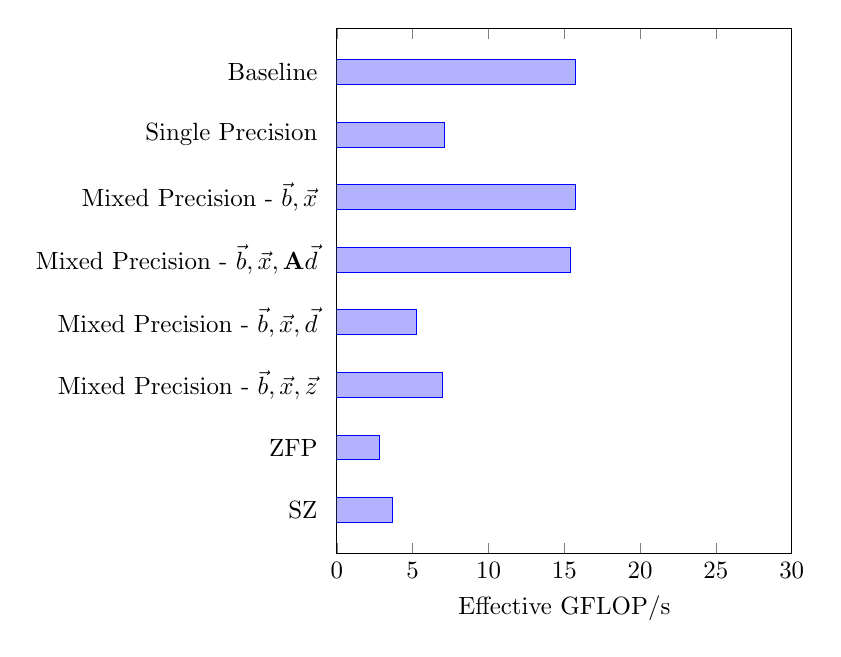
\begin{tikzpicture}[scale=.9]
		\begin{axis}[xbar,
					xlabel={Effective GFLOP/s},
					xmin=0,
					xmax=30,
					width=8cm,
					height=9cm,
					ytick style={draw=none},
					symbolic y coords={{SZ},{ZFP},{Mixed Precision - b,x,z},{Mixed Precision - b,x,d},{Mixed Precision - b,x,Ad},{Mixed Precision - b,x},{Single Precision},{Baseline}},
					ytick={{SZ},{ZFP},{Mixed Precision - b,x,z},{Mixed Precision - b,x,d},{Mixed Precision - b,x,Ad},{Mixed Precision - b,x},{Single Precision},{Baseline}},
					yticklabels={{SZ},{ZFP},{Mixed Precision - \(\vec{b}, \vec{x}, \vec{z}\)},{Mixed Precision - \(\vec{b}, \vec{x}, \vec{d}\)},{Mixed Precision - \(\vec{b}, \vec{x}, \mat{A}\vec{d}\)},{Mixed Precision - \(\vec{b}, \vec{x}\)},{Single Precision},{Baseline}} ]
			\addplot coordinates{
				(15.7394,Baseline)
				(7.10126,Single Precision)
				(15.7503,{Mixed Precision - b,x})
				(15.4048,{Mixed Precision - b,x,Ad})
				(5.25084,{Mixed Precision - b,x,d})
				(6.98823,{Mixed Precision - b,x,z})
				(2.80692,ZFP) %3d 14 bit
				(3.69907,SZ) %24 vals/block
			};
		\end{axis}
	\end{tikzpicture}
\end{frame}

\begin{frame}
	\frametitle{Matrix Value Compression}
	\raggedleft
	\begin{tikzpicture}[scale=.9]
		\begin{axis}[xbar,
					xlabel={Effective GFLOP/s},
					xmin=0,
					xmax=30,
					width=8cm,
					height=9cm,
					ytick=data,
					ytick style={draw=none},
					yticklabels from table={\valtable}{graphname},
					y dir=reverse]
			\addplot table[x=gflops,y expr=\coordindex]{\valtable};
		\end{axis}
	\end{tikzpicture}
\end{frame}

\begin{frame}
	\frametitle{Matrix Index Compression}
	\raggedleft
	\begin{tikzpicture}[scale=.9]
		\begin{axis}[xbar,
					xlabel={GFLOP/s},
					xmin=0,
					xmax=30,
					width=8cm,
					height=9cm,
					ytick=data,
					ytick style={draw=none},
					yticklabels from table={\indtable}{graphname},
					y dir=reverse]
			\addplot table[x=gflops,y expr=\coordindex]{\indtable};
		\end{axis}
	\end{tikzpicture}
\end{frame}

\begin{frame}
	\frametitle{Matrix Value and Index Compression}
	\raggedleft
	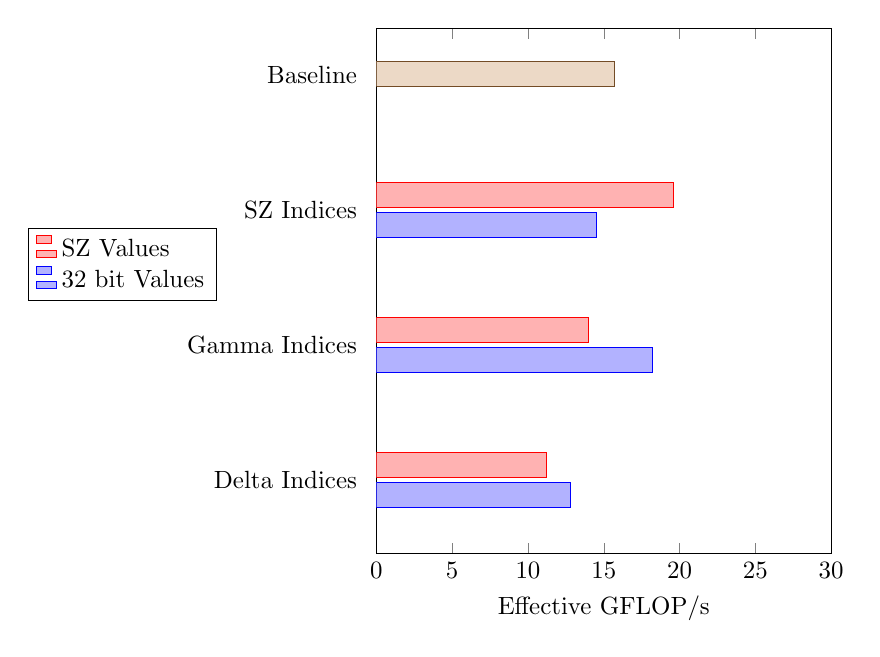
\begin{tikzpicture}[scale=.9]
		\begin{axis}[xbar,
					xlabel={Effective GFLOP/s},
					xmin=0,
					xmax=30,
					width=8cm,
					height=9cm,
					enlarge y limits=0.25,
					y dir=reverse,
					ytick style={draw=none},
					ymax=2.9,
					ymin=.3,
					ytick            ={0,1,2,3},
					yticklabels={{Baseline},{SZ Indices},{Gamma Indices},{Delta Indices}},
					legend style={
						anchor=east,
						at={(axis description cs:-.35,.55)}
					},
					legend cell align=left,
					reverse legend,
				]
			\addplot coordinates{% 32 bit vals
				(14.5156,1)
				(18.1835,2)
				(12.8181,3)
			};
			\addlegendentry{32 bit Values}
			\addplot coordinates{% SZ vals
				(19.5759,1)
				(13.9794,2)
				(11.1961,3)
			};
			\addlegendentry{SZ Values}
			%don't add to legend, but use the third bar styling
			\addplot[forget plot, brown!60!black,fill=brown!30!white,mark=none] coordinates{%baseline
				(15.7394,.32)
			};
		\end{axis}
	\end{tikzpicture}
\end{frame}

\begin{frame}
	\frametitle{Vector and Matrix Compression}
	\raggedleft
	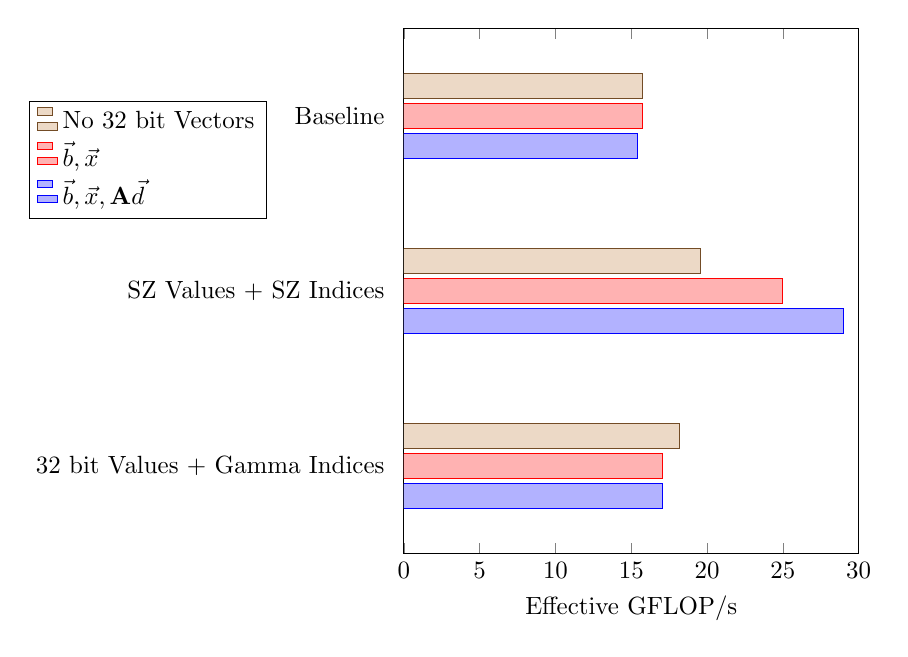
\begin{tikzpicture}[scale=.9]
		\begin{axis}[xbar,
					xlabel={Effective GFLOP/s},
					xmin=0,
					xmax=30,
					width=8cm,
					height=9cm,
					y dir=reverse,
					ytick style={draw=none},
					symbolic y coords={Baseline,SZ,Gamma},
					ytick            ={Baseline,SZ,Gamma},
					yticklabels={{Baseline},{SZ Values + SZ Indices},{32 bit Values + Gamma Indices}},
					enlarge y limits=0.25,
					legend entries={{\(\vec{b},\vec{x},\mat{A}\vec{d}\)},{\(\vec{b},\vec{x}\)},{No 32 bit Vectors}},
					reverse legend=true,
					legend style={
						anchor=east,
						at={(axis description cs:-.3,.75)}
					},
					legend cell align=left,
					]
			\addplot coordinates{ %b,x,Ad single
				(15.4048,Baseline)
				(28.9699,SZ)
				(17.02944,Gamma)
			};
			\addplot coordinates{ %b,x single
				(15.7503,Baseline)
				(24.9875,SZ)
				(17.0684,Gamma)
			};
			\addplot coordinates{ %no single
				(15.7394,Baseline)
				(19.5759,SZ)
				(18.1835,Gamma)
			};
		\end{axis}
	\end{tikzpicture}
\end{frame}

% Conclusion
\begin{frame}
	\frametitle{Conclusion}
	\begin{itemize}
		\item Iterative, sparse linear solvers are memory access bound
		\item Compressing key data structures provided an 84\% increase in performance
	\end{itemize}
\end{frame}

\end{document}
